\documentclass[10pt,onecolumn]{article}
\usepackage{graphicx}
\usepackage{hyperref}

\title{\vspace{-4.2cm}Software Requirement Specification for Tracking Interconnected Facebook Links }
\author{ ELEN4009 - Software Engineering\\ Julian Zeegers (704582) \\  Joseph Gage (751052)\\ James Allingham (672732) \\ Nathan Haag (873666)}

\addtolength{\oddsidemargin}{-1.5cm}
\addtolength{\evensidemargin}{-.0cm}
\addtolength{\textwidth}{3cm}


%%%%%%%%%%%%%%%%%%%%%%%%%%%%%%%%%%%%%%%%%%%%%%%%%%%%%%%%%%%%%%%%%%%%%%%%%%%%%%%
\begin{document}
\date{\vspace{-5ex}}
\maketitle
\pagestyle{plain}
\setcounter{page}{1}

%%%%%%%%%%%%%%%%%%%%%%%%%%%%%Main Body%%%%%%%%%%%%%%%%%%%%%%%%%%%%%%%%%%%%%%


\section{Introduction}
The Tracking Interconnected Facebook Links project is a project that  is intended to visualize the links and connections of a Facebook user with other users. Initially, these visualization are focused on identifying the relationships of a Facebook user (and the end user of this product) with the network of friends this Facebook user has. The visuals are also intended to further illustrate the relationship connections of the users friends of friends and an overview of the user's friend network. There will be more features that could potentially be added to this tool and therefore the solution must be dynamic and flexible. This document describes the software requirements that will ensure that the end product is of the highest quality, produced most efficiently and is created as close to the requirements as possible.

\subsection{System Overview}
This project will be made up of various software systems with the back-end and front-end working together to form a dynamic visualization program. The overview of the entire software system is illustrated in Figure 1. This figure shows how the various components of the system interact with each other. Figure 1 shows how the client (using a web browser) interacts with an Apache server and the Django framework. It also shows that the Neo4j database provides data to the framework and is then sent to the web browser (through the Apache server) to create visualizations.

\begin{figure}[h]
	\centering
	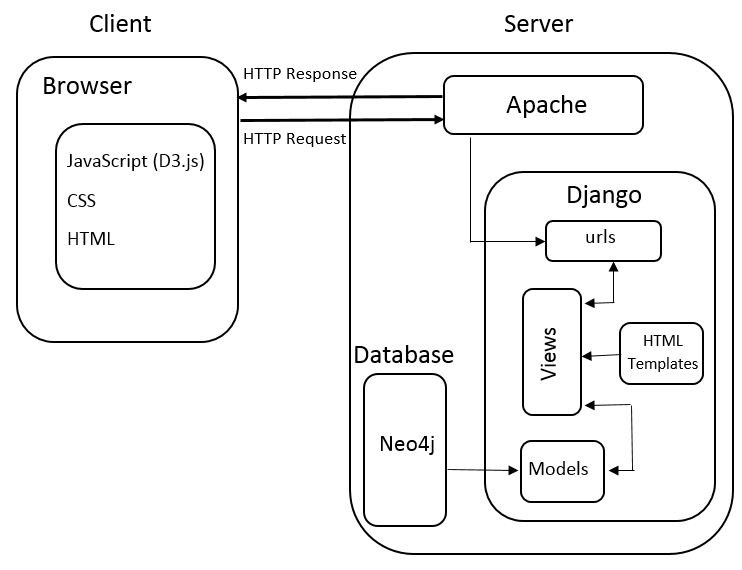
\includegraphics[scale=0.65]{system.jpg}
	\caption{Diagram of System Overview}
	\label{system}
\end{figure}

\section{Software Development Life Cycle Choice}
The Software Development Life Cycle (SDLC) is the process or approach the software development team adheres to throughout the project's development. Choosing the correct SDLC of the project is an important decision at the start of a software project as it could determine whether a project is successfully completed in the time given and at the required quality. There are a few SDLCs that are taken under consideration such the sequential development Waterfall approach or the Iterative and Incremental process in which features are gradually added. However, for this particular project, the fast pace method of the Agile SDLC was thought to be the best approach as the pace of producing a working solution is a priority. The requirements for this project is also not fully defined and therefore the chosen Agile SDLC must be flexible and able to deal with slight requirement changes.

The Agile SDLC also has varying methodologies that allows the achievement of an agile software development movement. These methods include the Dynamic System Development Method, the Scrum Method and the Feature-Driven Development Method. The Scrum methodology is the chosen method for this project as it allows the project progression to be agile and flexible with continuous feedback sessions to ensure the requirements are dynamical followed\cite{Kinsey}.

In the Scrum process, prioritized project tasks (referred to as sprints) are defined in short daily meetings (typically 15 minutes) with all the project team members. These meetings allow the team to communicate project progress and identify the important features that need to be added in order to increase the project progress pace. For the Tracking Interconnected Facebook Links project, these sprints will allow for a working product to be produced in the shortest amount of time while additional features can be  added at a later stage. This process also allows the client to closely keep track of progress and adjust the requirements in order to produce the most high-grade product possible. The daily meeting process occurs for up to 30 days by which time the first release of the developed software should be ready.   


\section{Architecture Choice}

\section{Front-end User Interface Method}
\section{Back-end Service}
\section{Supporting Software}
The Interconnected Facebook Links project is intended to be used by a Facebook user and this user is assumed to not technically advanced. Therefore the final product needs to be user friendly and easy to use. The supporting software mentioned in this section describes the technologies that will be used to ensure the user-friendliness and functionality of the product is achieved. The framework and internal structure  of the project in terms of the architecture, front-end and back-end has been described in the previous sections. This section describes the software that will be used to support these mentioned structures.

In order to ensure that the end program is easy to use and looks professional, the visual design and theme needs to have a consistent, well designed layout and be visually attractive. Bootstrap is a HTML, CSS and JavaScript framework that allows this front-end visual design to be achieved \cite{Bootstrap}. Bootstrap provides various templates that will maintain the consistent theme throughout the final created website. It also provides navigational links for the website and the template is customizable so it can be used to create the desired theme. The Bootstrap template that will be utilized is the "dashboard template" as it has a good layout, navigational links and is visually attractive which is taken from \cite{Bootstrap}.

Another technology that will support the functionally of the website is the D3.js JavaScript graphical library (assessed from \cite{D3}). This library contains JavaScript code for many different visualization graphs that can be used to visualize the data stored in the Neo4j database. Considering that the requirements for this project is to visualize the interconnections, the "force-directed graph" from the d3.js library will be used. Due to the fact that the requirements are flexible, other graphs from the d3.js library can also be used to the further visualize the database if the requirements change. These other graphs include dynamic bar and line charts, geographical heatmaps and dc.js crossfilter graphs plus others that will be considered. 

\begin{thebibliography}{1}
	\bibitem{Kinsey} H. van Vliet, \emph{Software Engineering: Principles
		and Practice} Wiley, 2007
	
	\bibitem{Bootstrap}  \emph{Get Bootstrap - 3.3.6} assessed from: \url{www.getbootstrap.com}
	
	\bibitem{D3}  \emph{D3.js - Data Driven Documents} assessed from: \url{www.d3.com}
	
	
\end{thebibliography}

 %%%%%%%%%%%%%%%%%%%%%%%%%%%%%%%%%%%%%%%%%%%%%%%%%%%%%%%%%%%%%%%%%%%%%%%%%%%%%%
\clearpage
\end{document}